\chapter{INTRODUCTION}

\section{Theorem Environment}
Please define theorems with following macros in \texttt{global.tex}:
\begin{itemize}
\item \cs{nuaatheoremchapu}, the suffix stands for CHAPter Unified,
it produces two-level unique numbering (recommended?)
\item \cs{nuaatheoremchap}, the suffix stands for CHAPter,
it produces regular two-level numbering
\item \cs{nuaatheoremg}, the suffix stands for Global,
it produces one-level numbering
\end{itemize}

Here is the \autoref{def:bonus}.
\begin{definition}\label{def:bonus}
  Bonus points are extra gains.
\end{definition}

\section{Using Figure}
Take a look at the figure below, and the table of figures for the \autoref{fig:logo}.

\begin{figure}[H]
  \subfloat[Logo in PDF]{
\includegraphics[width=3cm]{nuaa-logo}}\quad
  \subfloat[Figure in TikZ]{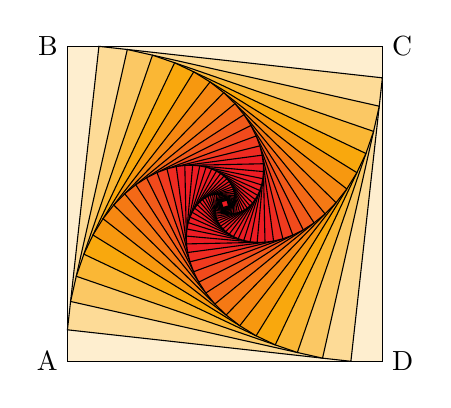
\begin{tikzpicture}
  \newcounter{density}
  \setcounter{density}{20}
  \def\couleur{Dandelion}
  \path[coordinate] (0,0) coordinate(A)
              ++( 90:4cm) coordinate(B)
              ++(0:4cm) coordinate(C)
              ++(-90:4cm) coordinate(D);
  \draw (A) node[left] {A}
    (B) node[left] {B}
    (C) node[right] {C}
    (D) node[right] {D};
  \draw[fill=\couleur!\thedensity] (A)--(B)--(C)--(D)--cycle;
  \foreach \x in {1,...,40}{%
      \pgfmathsetcounter{density}{\thedensity+25}
      \setcounter{density}{\thedensity}
      \path[coordinate] coordinate(X) at (A){};
      \path[coordinate] (A) -- (B) coordinate[pos=.1](A)
                          -- (C) coordinate[pos=.1](B)
                          -- (D) coordinate[pos=.1](C)
                          -- (X) coordinate[pos=.1](D);
      \draw[fill=\couleur!\thedensity] (A)--(B)--(C)--(D)--cycle;
  }
\end{tikzpicture}
}
  \caption[Demo]{This is a figure\label{fig:logo}}
\end{figure}

\section{Using Table}
Never underestimate the power of crowd (in bus/metro) as shown in \autoref{tab:city}.
\begin{table}[htb]
  \caption[City population]{City with large population (source: Wikipedia)\label{tab:city}}
  \begin{tabular}{lr}
    \toprule
    City & Population \\
    \midrule
    Mexico City & 20,116,842\\
    Shanghai & 19,210,000\\
    Peking & 15,796,450\\
    Istanbul & 14,160,467\\
    \bottomrule
  \end{tabular}
\end{table}

\section{Using Proof}
\begin{proof}
It is impossible to separate a cube into two cubes, or a fourth power into two fourth powers,
or in general, any power higher than the second, into two like powers.

I have discovered a truly marvelous proof of this, which this margin is too narrow to contain.
\end{proof}

\section{Using Reference}
Cite one paper\cite{r1}, or multiple\cite{r2,r3,r4}.

Here is inline cited paper\inlinecite{r6}, and another paper\inlinecite{r7,r8,r9}.

\section{Organization of the Thesis}
The organization of this thesis is as follows.
